\documentclass[deutsch]{llncs}
\usepackage{url}
\usepackage{graphicx}
\usepackage{listings}
\usepackage{verbatim}
\usepackage{listings}
\lstset{numberbychapter=false}
\usepackage[lined,linesnumbered,german]{algorithm2e}
\SetAlCapFnt{\small}
\SetAlCapNameFnt{\small}
\usepackage{tikz}
\usetikzlibrary{arrows,automata}
\usepackage{xspace}
% for german seminar theses
\usepackage[utf8]{inputenc}
\usepackage[ngerman]{babel}
\usepackage{csquotes}
\usepackage[abbreviate=false,maxbibnames=99,backend=bibtex]{biblatex}
\bibliography{referenzen}

\usepackage{hyperref}

\setcounter{secnumdepth}{2}
\setcounter{tocdepth}{3}

% define custom macros for specific formats or names
\newcommand{\uml}[1]{\texttt{#1}\xspace}
\newcommand{\cd}{\textsf{Klassendiagramm}\xspace}

% Numeriere 3 Ebenen tief (bis subsection)
\setcounter{secnumdepth}{2}

% make a proper TOC despite llncs
\setcounter{tocdepth}{2}
\makeatletter
\renewcommand*\l@author[2]{}
\renewcommand*\l@title[2]{}
\makeatletter

\begin{document}
\def\abstractname{Kurzfassung.}

\pagestyle{plain}
\pagenumbering{roman}

\title{Virtuelle und erweiterte Realität\thanks{Diese Arbeit wurde im Rahmen der LVA „Wissenschaftliches Arbeiten'' (188.925) im WS18 erstellt.}}


%&&&&&&&&&&&&&&&&&&&&&&&&&&&&&&&&&&&&&&&&&&&&&&&&&&&&&&&&&&&&&&&&&&&&&&&&
% Name and address of the author
%&&&&&&&&&&&&&&&&&&&&&&&&&&&&&&&&&&&&&&&&&&&&&&&&&&&&&&&&&&&&&&&&&&&&&&&&
%\author{Max Mustermann}

%\institute{Technische Universität Wien\\ Bachelorstudium Wirtschaftsinformatik\\ \email{max.mustermann@tuwien.ac.at} \\ Matrikelnr.: 0123456}

%&&&&&&&&&&&&&&&&&&&&&&&&&&&&&&&&&&&&&&&&&&&&&&&&&&&&&&&&&&&&&&&&&&&&&&&&
% Example for more than one authors
%&&&&&&&&&&&&&&&&&&&&&&&&&&&&&&&&&&&&&&&&&&&&&&&&&&&&&&&&&&&&&&&&&&&&&&&&
\author{Barbara Elias\inst{1} \and Yi Wang\inst{2}}

\institute{Technische Universität Wien\\ Bachelorstudium Medizinische Informatik\\ \email{e1028094@student.tuwien.ac.at} \\ Matrikelnr.: 01028094
\and
Technische Universität Wien\\ Bachelorstudium Wirtschaftsinformatik\\ \email{e1633407@student.tuwien.ac.at} \\ Matrikelnr.: 01633407}

\maketitle

% reset footnote counter in case of multiple authors
\setcounter{footnote}{0}

\begin{abstract}
Diese Arbeit beschäftigt sich mit dem Thema „virtuelle und erweiterte Realität'' insbesondere zu Ausbildungszwecken. Im Speziellen werden Publikationen von Mag. Dr. Hannes Kaufmann zur näheren Erarbeitung der Nutzung erweiterter Realität im Hinblick auf den Geometrieunterricht herangezogen. Seine Arbeiten zielen darauf ab, Geometrie begreifbarer zu machen, als es mit der Konstruktion mit Papier und Bleistift möglich ist. Basierend auf schon vorhandener Geometriesoftware wurden VR-Anwendungen konstruiert, die Mathematik verständlicher machen sollen. Die Idee dabei ist, den Schülerinnen und Schülern die Möglichkeit zu geben, mittels VR-Brille um dreidimensionale Objekte zu gehen und diese von neuen, ungeahnten Perspektiven erkennen zu können. Damit wird ein besseres Verständnis für räumliche Geometrie ermöglicht.
\end{abstract}

%&&&&&&&&&&&&&&&&&&&&&&&&&&&&&&&&&&&&&&&&&&&&&&&&&&&&&&&&&&&&&&&&&&&&&&&&
% Table of contents
% Activate or deactivate this according to the guideline instructor
%&&&&&&&&&&&&&&&&&&&&&&&&&&&&&&&&&&&&&&&&&&&&&&&&&&&&&&&&&&&&&&&&&&&&&&&&
\tableofcontents
\newpage
\pagenumbering{arabic}
\section{Einleitung}
\label{sec:intro}
Die Geschichte der virtuellen Realität reicht länger zurück als man auf den ersten Blick glauben möchte. Schon analoge Systeme der virtuellen Realität lassen sich finden. Diese sind zu Trainingszwecken im militärischen Bereich eingesetzt worden \cite{vrnerds}.
Mittlerweile finden sich zahlreiche Anwendungen der virtuellen und erweiterten Realität auch im Alltag: beispielsweise als Flugsimulatoren, in der Spieleindustrie (Konsolenspiele), in der Medizin zur Unterstützung bei Operationen und zu Therapiezwecken, auch im psychotherapeutischen Bereich oder aber um Lernstoff im wahrsten Sinn des Wortes „begreifbar'' zu machen \cite{Klampfer}. 
Flugsimulatoren dienen als frühes Beispiel für die Ausbildung und das Training von Piloten und Pilotinnen, das mit virtuellen Systemen realisiert wurde  \cite{Klampfer}.\\

Diese Arbeit beschäftigt sich mit dem Thema „virtuelle und erweiterte Realität", insbesondere damit, wie sich Anwendungen der erweiterten und virtuellen Realität in der Aus- und Weiterbildung nutzen lassen. 
Zunächst gilt es aber zu erklären, was sich hinter den Begriffen „virtuelle Realität'' und „erweiterte Realität'' verbirgt. 
Beispielsweise findet man sogenannte VR-Brillen, mit denen man Computerspiele ganz neu erleben kann.
\label{sec:typo}
Unter virtueller Realität (Virtual Reality, VR) wird eine computergenerierte Welt verstanden, die in Echtzeit von der benutzenden Person erforscht und erlebt werden kann, und alle physikalischen Eigenschaften wahrheitsgetreu abbilden kann. 
Augmented Reality (AR, bzw. erweiterte Realität) vermischt virtuelle Realität und physische Realität. Im Gegensatz zur virtuellen Realität ist die benutzende Person hier nicht von ihrer Umwelt abgegrenzt.
Als Beispiele für erweiterte Realität kann hier ``Google glass'' genannt werden. 
Um sich unter erweiterter Realität etwas vorstellen zu können, nennt man am besten Spiele wie ``Pokemon Go"  von Nintendo \cite{Klampfer}. Im Folgenden werden VR und AR im Einzelnen erläutert.\\


Virtuelle Realität soll der benutzenden Person idealweise ermöglichen, in der simulierten Realität so zu agieren, wie sie in der realen Welt gewöhnt ist\cite{vr}. Dabei spielen nicht nur visuelle Eindrücke, sondern auch akustische und gelegentlich taktile Wahrnehmungen eine Rolle \cite{vr}. Der Effekt, sich in einer virtuellen Umgebung einzutauchen und diese als real zu empfinden, nennt man Immersion \cite{vr}. Immersion resultiert aus vielen Einflussfaktoren \cite{vr}. Einer davon ist die Anpassungsfähigkeit des Systems an der benutzenden Person \cite{vr}. Bei der Interaktion ist es unabdingbar, dass der Input und die Reaktion des Systems zeitlich übereinstimmend stattfinden \cite{vr}. Dazu sind die physiologischen Rahmenbedingungen der Menschen von Bedeutung \cite{vr}. Beispielsweise, damit eine optische Perzeption wirklichkeitsgetreu erscheinen kann, ist die Erreichung einer Bildwiederholrate von geringstenfalls 15 - 20 Hz vorauszusetzen \cite{vr}. Da die Interaktivität sehr wichtig ist, zählt die Reaktionszeit zu den Auswahlkriterien der Hardware- und Software-Elemente \cite{vr}. Weitere wichtige Komponenten der Immersion sind beispielsweise die Positionsverfolgung und Orientierung \cite{vr}. Das System koordiniert stets die optische und auditive Ausgabe mit der momentanen Orientierung \cite{vr}. Dies trägt zur Stabilisierung der Immersion bei \cite{vr}.
Ein VR-System muss die technischen Anforderungen an eine Schnittstelle zwischen Menschen und Maschine erfüllen, welches auch für ein AR-System gilt \cite{Klampfer}. Um dies zu erreichen, sind neben dem Computersystem mit entsprechender Software auch die folgenden Ausgabe- und Eingabegeräte unerlässlich: 
Als Ausgabegeräte für VR kommen Head-Mounted-Displays in Frage, welche auch für erweiterte Realität verwendet werden können. Weiters wird auch haptisches Feedback benötigt, beispielsweise Windgeneratoren oder sich bewegende Plattformen \cite{Klampfer}. 
Um die genaue Position eines Benutzers oder einer Benutzerin im Raum zu erkennen und im Rechner erfassen zu können, werden am besten möglichst viele Daten der benutzenden Person benötigt, die über die Erfassung von Finger-, Augen-, oder Kopfbewegungen eingespeist werden\cite{Klampfer}. Dazu kann sogar Ultraschall zum Einsatz kommen\cite{Klampfer}. Momentan wird aber überwiegend in Richtung des optischen Erfassens entwickelt \cite{Klampfer}.\\

Erweiterte Realität ist eine Technologie, die es ermöglicht, computergenerierte virtuelle Bildinformationen in Echtzeit einer direkten oder indirekten realen Umgebung zu überlagern \cite{Edu}. AR unterscheidet sich von virtueller Realität (VR) dadurch, dass in VR erwartet wird, dass Menschen eine computergenerierte virtuelle Umgebung erleben \cite{Edu}. In AR ist die Umgebung real, aber erweitert um Informationen und Bilder aus dem System \cite{Edu}. Mit anderen Worten, AR schließt die Lücke zwischen dem Realen und dem Virtuellen auf nahtlose Weise \cite{Edu}.\\
Die Geschichte von AR geht auf die 1960er Jahre zurück \cite{Edu}. Das erste System wurde von Ivan Sutherland kreiert, ist sowohl für AR als auch für VR relevant \cite{Edu}. Dabei wurde ein optisches, durchsichtiges und kopfgetragenes Display eingesetzt, das mit einer von zwei verschiedenen Methoden verfolgt wurde: einem mechanischen Tracker und einem Ultraschalltracker\cite{Edu}. Aufgrund der damals begrenzten Rechenleistung von Computern konnten nur sehr einfache Drahtgitter-Zeichnungen in Echtzeit dargestellt werden \cite{Edu}. Seitdem wird AR von einer Reihe großer Unternehmen für Visualisierung, Schulung und andere Zwecke eingesetzt \cite{Edu}. Der Begriff ``Augmented Reality" wird dem ehemaligen Boeing-Forscher Tom Caudell zugeschrieben, der den Begriff vermutlich 1990 geprägt hat\cite{Edu}.

Es gibt mehrere Möglichkeiten, wie die virtuellen Komponenten und realen Inhalte zur Interaktion gebracht werden können \cite{mullen_2011}. Mit Techniken der Bildverarbeitung und Computer-Vision können die computergenerierten Elemente mit dem realen Inhalt interagieren \cite{mullen_2011}. Die meisten aktuellen computerbildbasierten Verfahren basieren auf vordefinierten physikalischen Markern, damit sich das Computerbildsystem im sichtbaren 3D-Raum orientieren kann \cite{mullen_2011}. AR-Systeme können markerbasiert oder markerlos basierend sein \cite{Edu}. Markerbasierte Anwendungen funktionieren mit visuellen Markern, z.B. 2D-Barcodes, die mit computergestützten Bildverarbeitungsmethoden erkannt werden können \cite{Edu}. Hingegen benötigen markerlose Anwendungen ein Ortungssystem, das beispielsweise GPS (\emph{Global Positioning System}), einen Kompass und ein Bilderkennungsgerät beinhaltet \cite{Edu}. Markerlose Anwendungen haben eine breitere Anwendbarkeit, da sie überall funktionieren, ohne dass spezielle Kennzeichnungen oder zusätzliche Referenzpunkte erforderlich sind\cite{Edu}. ``Pokemon Go'' ist ein Beispiel dafür.\\
Augmented-Reality-Systeme erfordern derzeit sowohl Hardware als auch Software, um ein überzeugendes AR-Erlebnis zu realisieren\cite{craig_2013}. Sensoren, Prozessoren und Display sind die drei hardware-technisch gesehenen Kernelemente eines AR-Systems\cite{craig_2013}. Die Software-Komponenten sind sehr vielfältig: sei es die Software, die tatsächlich zum Zeitpunkt der Nutzung der AR-Anwendung läuft, oder die Software, die zur Erstellung von Inhalten für eine AR-Anwendung verwendet wird\cite{craig_2013}. Für AR-Entwickler/in gibt es viele leistungsfähige Tools und AR-Bibliotheken\cite{craig_2013}. Nicht nur die Software- und Hardware-Komponenten, sondern auch andere wie beispielsweise Interaktion oder Inhalt müssen zusammenwirken, um ein erfolgreiches System zu sein \cite{craig_2013}.\\

\emph{``Mobile augmented reality“} ist beispielsweise derzeit eines der explosivsten Wachstumsfelder für AR-Anwendungen\cite{craig_2013}. Weitere Einblicke in State of the Art bzw. Einsatzgebiete von VR und AR werden im Kapitel 2 gewährt. Im Kapitel 3 handelt es sich um die Arbeiten von Dr. Hannes Kaufmann, die eine VR/AR-Anwendung für den Geometrieunterricht thematisieren. Während eine Zusammenfassung im Kapitel 4 zu finden ist, enthält das Kapitel 5 das Literaturverzeichnis.

\section{Einsatzgebiete}
Erweiterte und auch virtuelle Realität haben mittlerweile Einzug in viele Bereiche des täglichen Lebens gehalten, wobei sich eine Tendenz in Richtung erweiterte Realität erkennen lässt. Einer der Vorteile für den praktischen Einsatz von erweiterter Realität wäre zum Beispiel, dass die tatsächlich vorhandene Realität mit der, der virtuellen verbindet wird. Dies hat beispielsweise in der Medizin bereits zu einigen sinnvollen Anwendungen geführt. Im Folgenden werden einige Einsatzgebiete von sowohl erweiterter, als auch virtueller Realität näher beschrieben: 
\begin{itemize}
\item Medizin \& Psychotherapie:\\
Am medizinischen Sektor gibt es schon einige Anwendungsmöglichkeiten: beispielsweise in der Tumorentfernung, bei der Behandlung von Phantomschmerzen, bei der Traumabewältigung oder Hilfe bei der Überwindung von Höhenangst. 
Ein Beispiel zur Anwendung bei Phantomschmerzen: Wurde jemandem eine Extremität entfernt, kann es passieren, dass das Schmerzzentrum des Gehirns immer noch Schmerzen vom bereits entfernten Körperteil wahrnimmt. Bisher wurde gute Ergebnisse in der Therapie mit der sogenannten Spiegeltherapie erzielt. Diese Methode wurde mithilfe von virtueller Realität noch ausgebaut. Man lässt die zu therapierenden Personen durch eine VR-Brille schauen und visualisiert ihre fehlende Extremität mithilfe des Computers. Das Gehirn lernt damit, dass die Schmerzen nicht notwendig sind, weil das fehlende Körperteil ohnehin noch da zu sein scheint \cite{psycho}.  \\
Ebenso ist es bereits möglich, das Bild eines Tumors überlagernd auf das Organ eines/einer Patienten/in zu projizieren, damit der/die Chirurg/in die Größe des Tumors visualisieren kann.
\item Erweiterte Realität im Museum: \\
Mittels spezieller Brillen, die im Museum angeboten werden, können die Informationen zu den Exponaten den Museumsbesuchern und Museumsbesucherinnen direkt auf einer eigens abgestimmten AR-Brille gezeigt werden. 
\item Erweiterte Realität für die Automechaniker/innen:\\
Automechaniker/innen können sich bei der Zerlegung eines Motorblocks die einzelnen Schritte über eine Brille anzeigen lassen und auch das entsprechende Werkzeug einblenden lassen. 
\item Marketing: \\
Ebenso in diesem Bereich halten sowohl die virtuelle als auch die erweiterte Realität immer mehr Einzug. Es geht heutzutage nicht nur um den Produktverkauf, sondern um das Erlebnis, das der Kunde oder die Kundin spüren möchte. Interaktive Showrooms bieten den Kund/innen das ultimative Shoppingerlebnis \cite{}.

\end{itemize}
\subsection{Aus- und Weiterbildung}
Seit den frühen 1990er Jahren wird an Software für den Einsatz in der Aus- und Weiterbildung geforscht. Im Feld der Mathematik kann hier als herausragendstes Projekt ``CyberMath'' genannt werden. CyberMath verwendet eine virtuelle Lernumgebung, die mittels Avataren gesteuert werden kann. \\
VR und AR-Systeme generieren einen ganz neuen Zugang zum Lernen, weg von den gewöhnlichen traditionellen Methoden. Dies spiegelt das Prinzip modernes Lernens wieder. Denn modernes Lernen heißt, dass Wissen basierend auf authentischen Situationen vermittelt wird und der oder die Lernende im Mittelpunkt steht \cite{Klampfer,unknown}.

Aufgrund der Entwicklung bzw.Verbesserung der Informationstechnologie haben VR/AR-Anwendungen nun in der allgemeinen und beruflichen Bildung einen effizienteren Ansatz mit einer breiteren Benutzerakzeptanz als je zuvor \cite{Edu}. Es ist auch möglich, diese Anwendungen mit den drahtlosen Mobilgeräten wie Smartphones, Tablet-PCs und anderen elektronischen Innovationen zu realisieren \cite{Edu}. Der Tendenz zu mobilem Raum ist zu erkennen, in dem Anwendungen vielversprechend sind \cite{Edu}.
In den letzten Jahrzehnten haben viele Fachleute und Forscher/innen pragmatische Theorien und Anwendungen hinsichtlich der Aus- und Weiterbildung im verschiedenen Umfeld entwickelt\cite{Edu}. Einige Beispiele dazu werden nun aufgelistet:
\begin{itemize}
\item \emph{Augmented Chemistry} ist eine interaktive Lernwerkbank, die den Schüler/innen mittels AR zeigen kann, wie und woraus ein Atom oder ein Molekül besteht \cite{Edu}. Für die Umsetzung werden ein Booklet, ein Greifer und ein Würfel benötigt \cite{Edu}. Das Booklet dient zum Bereitstellen von Markerinformationen \cite{Edu}. Der Greifer hilft beim Abrufen von Informationen aus dem Booklet und deren Konvertierung in eine andere Art von Daten\cite{Edu}. Der Würfel wird fürs Erweitern von Informationen in 3D-gerenderte Informationen auf einem Bildschirm verwendet\cite{Edu}.
\item \emph{VRMagic EYESi®} ist ein ophthalmischer VR-Simulator, der für chirurgische Trainings bedacht ist \cite{augen}. Inkludiert sind neben dem Ophthalmoskop-Simulator für Netzhautuntersuchungstrainings auch Vitreoretinaltrainingsmodule (Operationstrainings am hinteren Augenabschnitt) und Katarakt(Grauer Star)-trainingsmodule\cite{augen}. Bisherige Studienergebnisse besagen, dass die Assistenzarztausbildung und deren Performance dadurch positiv beeinflusst wurden und somit eine Sicherheit im OP-Saal gewährt wurde\cite{augen}. 
\item \emph{VROnSite-Platform} ermöglicht ein kosteneffizientes, zeiteffizientes und realistisches Training von Einsatzleiter/innen der Feuerwehr und des Rettungsdienstes vor Ort\cite{Feuerwehr}. Immersive virtuelle Realität wird mit natürlichem Gehen kombiniert und zur Simulation von Entscheidungsprozessen unter Stress und Erschöpfung eingesetzt\cite{Feuerwehr}. 
\end{itemize}
Wie bereits zu erkennen ist, sind VR/AR-Anwendungen nicht nur für berufstätige Personen, sondern auch für Schüler/innen sehr relevant. 

\subsection{Lernen im Schulunterricht des 21. Jahrhunderts}
Schülerinnen und Schüler stellen immer mehr den Sinn dessen, was sie tagtäglich in der Schule lernen sollen, in Frage \cite{Klampfer}. Lehrerinnen und Lehrer wiederum sind oft überfordert damit, wie sie den vorgeschriebenen Unterrichtsstoff zeitgemäß nahe bringen können. Um Schüler/innen und Studierende zeitgemäß zu unterrichten, müssen sich neue Methoden formieren, bzw. haben sich bereits etabliert, da sonst Gefahr läuft, dass Lernende die Lust am Lernen verlieren. Im Moment existiert ein Trend, weg von Frontalvorträgen, die isoliert von ihrem Kontext vorgetragen werden, hin zum Einsatz von neuen Medien wie beispielsweise virtuelle Realität im Unterricht. Mehrere Studien \cite{Hu-Au} zeigen, dass damit der Einsatz und die Begeisterungsfähigkeit von Lernenden massiv gehoben werden können.
Mehrere Aspekte, wie beispielsweise pädagogische und psychologische, müssen im Vorfeld betrachtet werden, damit eine Software für Weiterbildungszwecke vernünftig und zielführend entwickelt werden kann \cite{article}.
\subsection{Von der Zweidimensionalität in die dritte Dimension}
%\label{subsec:}
Erfahrungsgemäß haben einige Schülerinnen und Schüler Probleme damit, sich geometrische Objekte, dargestellt auf Papier oder einer Schultafel vorzustellen und anhand dieser Skizzen mathematische Problemstellungen zu begreifen und zu lösen. Mit dem Einsatz von VR bzw. AR soll dieses Problem gelöst werden.\\
Software, um die Ideen und Grundlagen der Geometrie zu lehren, existiert bereits seit Anfang der 1990er, allerdings damals nur in 2D \footnote{GeoGebra, https://www.geogebra.org}. \\
\emph{Construct3D} ist die erste Software für die Aus- und Weiterbildung, die auch die dritte Dimension nutzt. %\cite{4}
%\newpage
\section{Virtuelle und erweiterte Realität im Geometrieunterricht}
%Babsis Implementierung der Papers starts here
\subsection{Motivation}
Auf der Basis, dass räumliches Vorstellungsvermögen einen wichtigen Teil menschlicher Intelligenz ausmacht \cite{spatial}, hat Hannes Kaufmann im Jahr 2002 seine Forschung auf dem Gebiet der virtuellen Realität begonnen.
Menschen leben in einer dreidimensionalen Welt und sind es gewohnt, Dinge von allen Seiten betrachten zu können. Daher ist es naheliegend, auch für den Geometrieunterricht ein System zu entwickeln,
das dem menschlichen Denken in dieser Hinsicht entgegenkommen soll. Im von Hannes Kaufmann untersuchten Fall war dies ein Tool, das sogenannte \emph{Construct3D}, auf das im Weiteren näher eingegangen wird. Dabei wird der Schwerpunkt auf 4 ausgewählte Artikel von Hannes Kaufmann geleget, nämlich:  \emph{``Mathematics and geometry education with collaborative augmented reality"}\cite{Kaufmann:2002:MGE:1242073.1242086}, \emph{``Collaborative augmented reality in education"}\cite{article}, \emph{``Designing immersive virtual reality for geometry education"} \cite{1667626} und \emph{``Summary of usability evaluations of an educational augmented reality application"}\cite{Kaufmann_summaryof}. \\

 Schon in früheren Untersuchungen wurde festgestellt, dass sich Geometrieunterricht positiv auf räumliche Intelligenz auswirkt \cite{GittlerDifferentialTO}.
Herkömmliche  \emph{computer-aided-design}(CAD)-Software  ist nicht gleichzusetzen mit der Implementierungsidee von Hannes Kaufmann. Denn im Unterschied zu CAD-Software, wird im Geometrieunterricht kein Wert darauf gelegt, feinsäuberliche Modelle zu kreieren, sondern auf die inhärente Konstruktion von geometrischen Objekten. Die kommerzielle CAD-Software, die verfügbar ist, ist meistens zu komplex und hat einen zu hohen Lernaufwand, um für den Geometrieunterricht in Frage zu kommen  \cite{Kaufmann:2002:MGE:1242073.1242086}. \\
Es muss sowohl bei Software als auch Hardware, die im Unterricht verwendet werden soll, bedacht werden, dass Schulen nicht den finanziellen Aufwand aufbringen können, der für eine Versuchsumgebung in der Forschung verwendet werden kann.  Die Technologie, die hier entwickelt wurde, soll zukünftig selbstverständlich keine Lehrenden ersetzen, sondern als Mittel zur Unterstützung im Unterricht gesehen werden \cite{article}. Dies wird in der wissenschaftlichen Fragestellung von Hannes Kaufmann indiziert: \emph{``Our ultimate pedagogic goal is to verify if working directly in 3D space allows better and faster comprehension of complex spatial problems and relationships than traditional teaching methods."} \cite{1667626}. \\
\subsection{Entwicklung des vr/ar-basierten Lernsystems \emph{Construc3D} }
\textbf{Der technische Aufbau} \\
Ausgangspunkt für die Forschung ist die Software \emph{Construct3D}, die mehrere Komponenten vereint: Geometrie, Pädagogik, Psychologie und erweiterte Realität \emph{augmented reality (AR)}.
Basierend auf dieser schon existierenden Software, hat Hannes Kaufmann seine Forschungsumgebung eingerichtet \cite{Kaufmann:2002:MGE:1242073.1242086}. 
Weiters wurde ein System namens \emph{Studierstube} eingesetzt, welches mehreren Benutzerinnen und Benutzern erlaubt, einen gemeinsamen virtuellen Raum zu nutzen.
In einer frühen Phase von \emph{Construct3D} war es möglich primitive Funktionen wie beispielsweise Punkte, Linien, Zylinder und Kegel anzubieten.
Ein weiteres Werkzeug, \emph{OpenCascade}, bietet die Möglichkeit auch Boolesche-Operationen durchzuführen.
An Hardware stehen \emph{Head-mounted-Displays (HMDs)}, konventionelle Monitore und diverse Eingabegeräte zur Verfügung. Um Buttons, Sliders sowie andere Elemente in üblicher 2D-Grafik zu integrieren, existiert noch ein \emph{PIP}(\emph{personal interaction panel})  zusätzlich, um haptisches Feedback für die Benutzenden zu simulieren. Weiters werden Kopf und Hände mit einem ARTTrack1 Tracking-System verfolgt.
Die Umsetzung mittels AR bietet der Benutzerin/dem Benutzer die Möglichkeit, den eigenen Körper und die daraus folgende Beziehung im Raum zu den virtuell-erzeugten geometrischen Objekten besser wahrzunehmen. 
Ein aus mehreren Ebenen bestehendes System, ähnlich zu bekannter Photobearbeitungssoftware, wird verwendet, um Überlappungen in der Konstruktion der Objekte realistisch und verständlich darzustellen. Dies dient auch dazu, dass mehrere Benutzerinnen und Benutzer jeweils eine eigene Ansicht nutzen können und auch die Lehrer-Schüler-Interaktion besser abgebildet werden kann. 
Drei mögliche Benutzermodi (alle sehen alles, jeder und jede der Lernenden sehen nur die eigenen Konstruktionen oder ein lehrender Modus) existieren in einer frühen Version. \\
In weiterer Entwicklungsarbeit wurden im Jahr 2003 neue Lernmodi eingeführt, die im Folgenden näher beschrieben werden:
 \\
\begin{itemize}
\item \emph{Teacher-mode}:
Ein Lehrer oder eine Lehrerin kann in diesem Modus einen oder mehrere Lernende unterrichten, indem er/sie eine komplette Konstruktion mit all ihren Einzelschritten vorgibt. 
\item \emph{Normal tutorial}:
Hier wird den Lernenden ein Videotutorial mit allen notwendigen Schritten gezeigt, die diese dann reproduzieren sollen. 
\item \emph{Auto-tutorial}:
Schülerinnen und Schüler können sich selbstständig mit den einzelnen Schritten beschäftigen und mittels \emph{text-to-speech} System Erklärungen anhören. 
\item \emph{Exam-mode}: 
Die Lernenden sollen hier ohne Anleitung selbst Konstruktionen bauen und können diese am Ende mit einer vorgebenen Lösung vergleichen \cite{article}. 
Um das Menü von \emph{Construct3D} auf den HMDs gut lesbar zu machen und das Menü zu simplifizieren, wurden im Jahr 2006 entsprechende Anpassung vorgenommen. Auch die Anzahl an Funktionen hat seit  der ersten Version im Jahr 2002 zugenommen, weshalb das Menü reorganisiert werden musste \cite{1667626}. \\\end{itemize}
\textbf{Visualisierungstechniken} \\
Zu den Visualisierungstechniken, die in \emph{Construct3D} verwendet werden, gehören die Verwendung von Transparenz, um das Verständnis für die Konstruktion zu verbessern, eine Farbcodierung zur Unterscheidung der Benutzer/innen, eine Trennung der Ebenen sowie eine automatische Vorschau neuer Objekte. Im Folgenden werden diese Techniken näher beschrieben. Derlei Anpassungen machen zwar Szenenverarbeitung und Rendering signifant teurer, was aber zugusnten der Benutzerfreundlichkeit gerne in Kauf genommen wurde \cite{1667626}. 
\begin{itemize}
\item Transparenz: 
Diese wird  immer wieder auch in technischen Zeichnungen und Computerspielen eingesetzt, um versteckte Objekte darzustellen. Mittels Transparenz lassen sich Tiefe und andere räumliche Beziehungen darstellen (siehe Abb.1). Erst sollten die Benutzer/innen selbst mittels Slider die transparenten Bereiche auswählen. Diese Idee wurde aber verworfen, da sie zu Verwirrungen geführt hatte. Transparenz erschwert auch den Prozess des Renderings, wodurch manche Objekte nicht mehr richtig dargestellt werden können\cite{1667626}. 
Es besteht daher die Möglichkeit für die Benutzer/innen, die Ansicht in den sogenannten \emph{Wireframe-mode} umzuschalten, was folglich bedeutet, dass nur eine Art von Gitternetz-System die Form des Objekts bzw. dessen Oberfläche markiert.  
\item Farbcodierung und Ebenensystem:
Um ein übersichtliches System über die Eingaben der benutzenden Personen zu behalten, wurde ein Ebenensystem mittels Aktiv- und Inaktiv-Modi mit Farbschemata eingeführt. Das umgesetzte System ist mit dem in der traditonellen Lehre vergleichbar, in der die Lehrkraft verschiedene Farben und Schattierungen an der Tafel verwenden kann, um unterschiedliche Ebenen herauszustreichen. In der virtuellen Umgebung können diese Ebenen zusätzlich je nach Bedarf zu- und weggeschaltet werden. \cite{1667626}. 
\item Vorschau und Highlighting:
Wenn eine Konstruktion mit den Eingabeparametern funktioniert, erfolgt eine visuelle Rückmeldung. Die Vorschaufunktion wird dann aktiviert, indem der Stift über ein Widget bewegt wird. Kommt der oder die Lernende mit dem Stift in die Nähe eines Objekts, wird dieses Objekt mit \emph{Wireframe-grid} hervorgehoben. Somit weiß die benutzende Person, dass dieses Objekt ausgewählt werden kann. Bei weiterem Nähern leuchtet die Farbe vom Objekt. Das deutet darauf hin, dass dieses Objekt nun im Raum bewegt werden kann\cite{1667626}.  
\end{itemize}
\begin{figure}[h]
%placing with [tb][h][t]
	\centering
	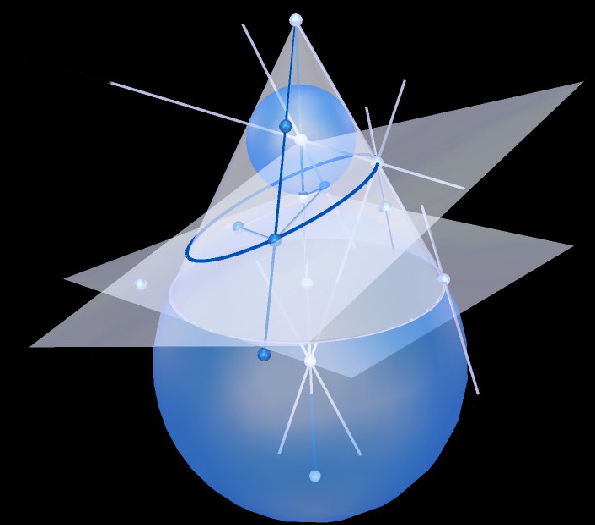
\includegraphics[width=0.7\textwidth]{figures/transparency}
	\caption{Erfolgreich dargestellte Transparenz \cite{1667626}}
	\label{fig:transparency}
\end{figure} 
 \textbf{Einsatz im Klassenzimmer} \\
Es wurden Rucksäcke mit Rechnern ausgestattet. Ein Tisch in der Mitte dient den Agierenden als Fixpunkt für die Zeichnungen. Alle Agierenden bekommen ein \emph{head-mounted-Display} (HMD) mit Kamera und Handschuhen als Eingabegerät. Da alles batteriebetrieben ist und somit keine Kabel notwendig sind, kann sich jeder/jede frei im Raum bewegen. 
Um mehrere Lernende partizipieren zu lassen, kann eine Projektion der Konstruktionen auf eine Tafel abgebildet werden. (Siehe \autoref{samplefigure}). \\
Das PIP (\emph{Personal Interaction Panel}) und ein dazugehöriger Stift ermöglichen die Eingabe sowohl im dreidimensionalen, als auch im herkömmlichen zweidimensionalen Stil \cite{1667626}. 

\begin{figure}[h]
%placing with [tb][h][t]
	\centering
	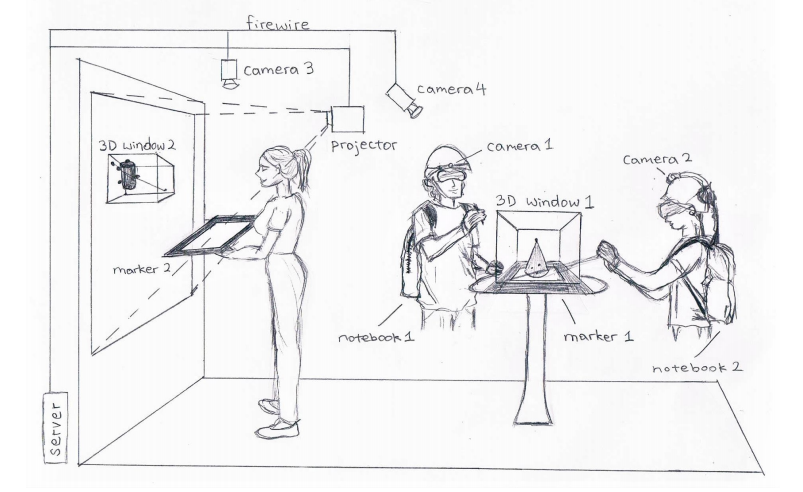
\includegraphics[width=1\textwidth]{figures/classroom}
	\caption{\emph{Augmented Classroom.} Bild nachgezeichnet basierend auf \cite{Kaufmann:2002:MGE:1242073.1242086} }
	\label{fig:samplefigure}
\end{figure}

%\subsection{Computergrafik know-how}
 Entwickelt und forscht man an der Darstellung von virtuellen Objekten im Raum, tauschen mitunter ungeahnte Schwierigkeiten auf, auf diese im Folgenden eingegangen wird.
\subsection{Statische und dynamische Geometrie}
Analysen aus den ersten Forschungsergebnissen haben gezeigt, dass es signifikant schwieriger als im zweidimensionalen Raum ist, vorgegebene Koordinaten in virtueller Realität zu finden und Punkte zu manipulieren. Aufgrund von Tremor (natürliches Zittern der Hände) und mangels Hand-Auge-Koordination ist es schwierig, einen Punkt genau zu treffen \cite{1667626}. 
Wie mehrere Studien zeigen, bietet es sich in manchen Situationen trotzdem an, auf eine zweidimensionale Darstellung zurückzukommen, da die 6 Freiheitsgrade in der Darstellung nicht immer von Vorteil sind \cite{Bowman:1999:ITC:930593}. 
Die exakte Eingabe von Koordinaten ist allerdings notwendige Voraussetzung, um mittels dynamischer Geometrie-Software starre Körper drehbar zu machen. Es sollte schließlich möglich sein, mehrere Objekte miteinander zu verbinden, um ,,was-wäre-wenn-Szenarios'' ausprobieren zu können. Mit traditionellen Methoden ist es wesentlich wichtiger, die Position des Objekts im Raum darstellen zu können. Dieser Aspekt verliert im dreidimensionalen Raum an Signifikanz \cite{1667626}. 
\subsection{Nebenwirkung - Simulator Sickness}
Ähnlich zu der schon bekannten Motion-Sickness \cite{motionsickness}, die manchmal bei Videospielen oder bei Reisen mit dem Auto, Zug oder Schiff auftritt, die zu Übelkeit und Schwindelgefühlen führen kann, da der Gleichgewichtssinn im Innenohr die Informationen, die die Augen liefern, nicht schnell genug verarbeiten kann, wird dieser gestört und so es kann auch beim Arbeiten mit \emph{Construct3D} zu einer Art Motion-Sickness, die hier allerdings
Simulatur Sickness genannt wird, kommen.
 \\
In der Evaluierung im Jahr 2003 wurde von einigen Lernenden über Simulator Sickness berichtet. 20 Minuten nach dem Beginn des Arbeitens in der virtuellen Umgebung tauchten Kopfschmerzen und Augenbelastungen bei einer Schülerin auf, trotzdem wollte sie damit weiterarbeiten. Nachträglich stellte sich heraus, dass die Zeiten für die kontinuierliche Arbeit mit einem HMD zu lang gewählt waren. Da negative Nebenwirkungen ein allgemeines potenzielles Problem bei der Arbeit mit HMDs darstellen und die subjektive Erfahrung der Nutzer/innen erheblich beeinflussen, sind sie für alle VR/AR-Anwendungen relevant, die diese Displays verwenden. Mögliche Gründe für diese Nebenwirkungen sind Akkomodationsprobleme, niedrige Bildfrequenz, Verzögerung oder schlechtsitzende Helme. 
Folglich wurde in der dritten Studie im Jahr 2005 die Trainingsdauer pro Einheit auf maximal 45 Minuten reduziert, der Hartplastikhelm durch einen leichteren Fahrradhelm ersetzt und von den Teilnehmenden selbstbestimmte Ruhezeiten eingeführt. Trotzdem spürten 75,56\% der 47 Teilnehmenden eine moderate Müdigkeit oder Erschöpfung und 61,36\% berichteten von einer leichten Augenbelastung. Einige hatten Kopfschmerzen (37,78\%) und Schwindelgefühl (35,56\%). Im Allgemeinen berichteten die meisten Teilnehmenden jedoch, dass sie keine schwerwiegenden Probleme hatten. Die meisten dieser Symptome könnten mit der Verwendung eines HMD zusammenhängen. In Übereinstimmung mit den Beobachtungen und anderen Studien wurde empfohlen, die HMD-Nutzungszeit auf 20-30 Minuten pro Einheit zu beschränken.  Basierend auf der Erfahrung trägt die Bildqualität von HMDs, insbesondere die Verzögerung und Qualität der Tracking-Daten, am meisten zu den berichteten Effekten bei \cite{Kaufmann_summaryof}.

\subsection{Evaluierungsergebnisse}
In der ersten Evaluierung im Jahr 2000 mit 14 Lernenden war eindeutig zu sehen, dass es nicht notwendig ist, den Schülerinnen und Schülern die Handhabung zu erklären. Die Bereitschaft besteht, eine Umgebung der erweiterten Realität zu benutzen. Es konnte beobachtet werden, dass alle Teilnehmenden stolz auf ihre Konstruktionen waren und freudig ihr Werk rundherum begutachteten. Die Hand-Auge-Koordination war in erster Instanz noch schwierig für die Versuchspersonen. Alle hatten Probleme damit, Punkte an vorgegebene Koordinaten richtig zu setzen, woraufhin zusätzlich ein Raster eingebaut wurde \cite{Kaufmann:2002:MGE:1242073.1242086}.\\

 Im Jahr 2003 wurde eine Studie auf Basis von Interviews und dem standardisierten Usability-Fragebogen ISONORM 9241/10 durchgeführt \cite{Kaufmann_summaryof}. Eine Reihe von Trainingsübungen wurde entwickelt, die zum österreichischen deskriptiven Geometrie-Curriculum der 11. und 12. Klasse passen \cite{Kaufmann_summaryof}.  Daran arbeiteten die Teilnehmenden (9 Schüler, 6 Schülerinnen) mit Hilfe ihrer Lehrenden. Jede Person nahm an 5 Trainingseinheiten mit einer Dauer von insgesamt 6 Stunden teil. Die Bewertung danach zeigte, dass die von Lernenden hoch bewerteten Kategorien (siehe Abb. \label{stat1}3) auch den subjektiv gesehenen höchsten Prioritäten einer Bildungsanwendung entsprechen (einfach bedienbar, schnell erlernbar; ermutigend, neues auszuprobieren; konsistent und im Gedächtnis bleibend)\cite{Kaufmann_summaryof}. Sowohl die ,,Eignung zum Lernen'' als auch die ,,Eignung zur Umsetzung der Aufgabe'' sind mit dem vorgegebenen Setting für die Testpersonen zur vollsten Zufriedenheit ausgefallen \cite{1667626}.
\begin{figure}[t]
%placing with [tb][h][t]
	\centering
	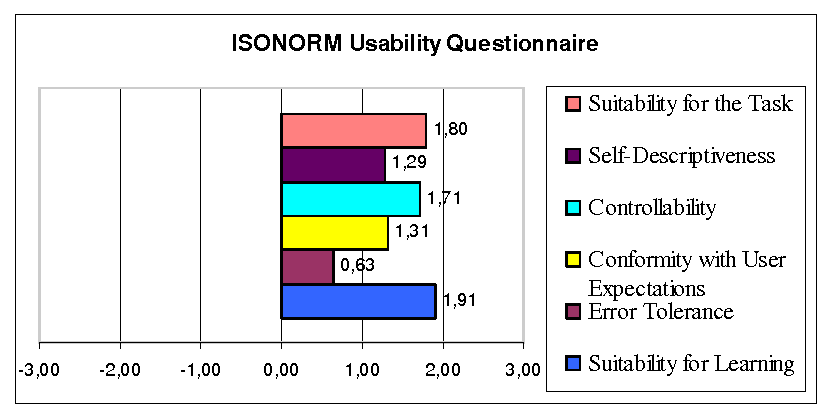
\includegraphics[width=0.9\textwidth]{figures/isonorm}
	\caption{Ergebnisse des ISONORM Usability-Fragebogens in 6 Kategorien \cite{Kaufmann_summaryof}}
	\label{fig:isonorm}
\end{figure}
\\Um die Selbstbeschreibbarkeit von \emph{Construct3D} zu verbessern, wurden bessere Beschriftungen hinzugefügt, sowie eine Hilfe-Box auf dem Panel, um alle Menüelemente zu erklären. Neben der neuen Strukturierung des Menüsystems wurde auch das visuelle Design von geometrischen Objekten verbessert  \cite{Kaufmann_summaryof}.  Eingeführt wurden Transparenz-Verwendung, konsistente Farbcodierung, Ebene-Trennung und automatische Vorschau neuer Objekte \cite{Kaufmann_summaryof}, wie es in \textbf{Visualisierungstechniken} vorgestellt wird.\\
Aus den Evaluierungsergebnissen von 2003 lassen sich folgende Aspekte ableiten: Von technischer Seite sind noch Probleme mit der Benutzerfreundlichkeit bezüglich Hard- und Software vorhanden. Die Orientierung zwischen Benutzenden und konstruiertem Objekt muss verbessert werden. Weiters können noch Verbesserungen im Bereich des Wohlbefindends bezüglich der Verwendung und des kognitiven Verständnisses der Lernenden stattfinden. Es lässt sich jedoch extrapolieren, dass ein messbarer Lernfortschritt mit der neuen Technologie erzielbar ist \cite{article}. \\

 Die dritte Auswertung war im Jahr 2005 \cite{Kaufmann_summaryof}. Verglichen wurde das Lösen von geometrischen Problemen mit \emph{Construct3D} mit einer pädagogischen Desktop-Anwendung namens CAD3D. Teilnehmenden waren österreichische Oberstufenschüler\_innen im Alter zwischen 16 und 19 Jahren (M = 17,49, SD = .79; 44 (48,4\%) männlich und 47 (51,6\%) weiblich) \cite{Kaufmann_summaryof}. Sie nahmen an 6 Trainingseinheiten teil, die 45 Minuten dauerten [4, S.665]. In beiden Gruppen betreute ein Tutor oder eine Tutorin zwei Lernenden beim Arbeiten an den Geometrieaufgaben  \cite{Kaufmann_summaryof}. Zur Beurteilung der Benutzerfreundlichkeit wurden Fragenbogen entwickelt, die von 8 etablierten Usability-Fragebögen angepasst waren (Siehe Abb. \label{stat1}4)  \cite{Kaufmann_summaryof}.
\begin{figure}[t]
%placing with [tb][h][t]
	\centering
	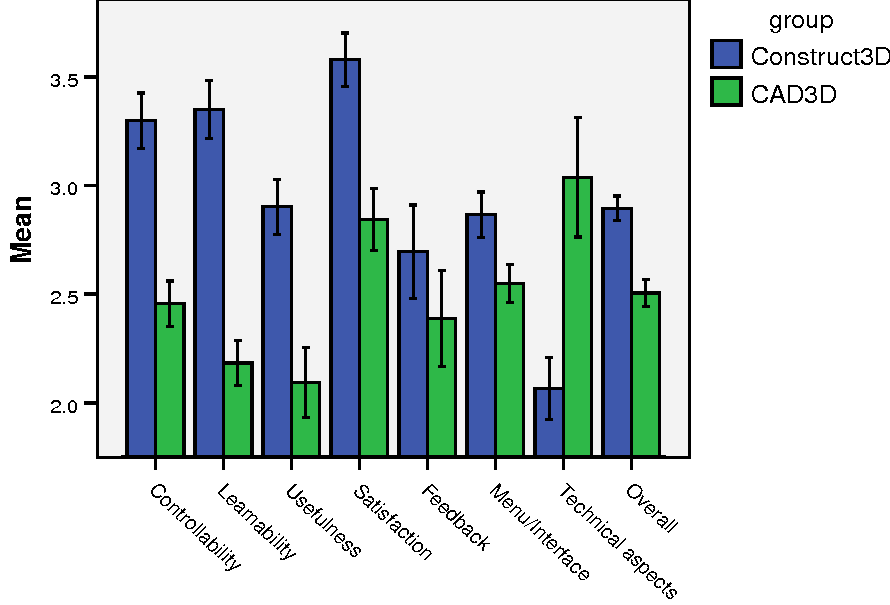
\includegraphics[width=0.9\textwidth]{figures/stat1}
	\caption{Usability-Bewertungen von Lernenden bezüglich der Verwendung von \emph{Construct3D} und CAD3D (4-Punkt-Likert-Skala; 1-min, 4-max = am besten; Fehlerbalken $\pm$ 1,96 * Standardfehler)\cite{Kaufmann_summaryof}}
	\label{fig:stat1}
\end{figure}
Die Analyse der Fragenbogen ergab, dass \emph{Construct3D} ein hochgradig benutzerfreundliches System ist, das - aus Usability-Sicht - mehrere Vorteile gegenüber der traditionellen Desktop-basierten Anwendung aufweist \cite{Kaufmann_summaryof}. Die niedrigen Bewertungen für technische Aspekte deuten jedoch darauf hin, dass es noch Probleme bezüglich der technischen Robustheit gibt, die angegangen werden müssen \cite{Kaufmann_summaryof}. Seltene Systemabstürze und kleinere technische Probleme können die Motivation der Teilnehmenden und die Benutzerfreundlichkeit des Systems beeinträchtigen. In Bezug auf die bevorzugte Trainingseinrichtung der Lernenden zwischen \emph{Construct3D} und CAD3D gab es keine signifikanten Unterschiede. Die Mehrheit der Lernenden möchte \emph{Construct3D} in der Schule einsetzen (ja = 64,44\%, eher ja = 26,67\%), 8,89\% möchten das System lieber nicht in der Schule einsetzen \cite{Kaufmann_summaryof}.  Die Kommentare zu den potenziellen Problemen beim Einsatz von \emph{Construct3D} in Schulen betrafen vor allem fehlende Finanzierung und die Robustheit der Hardware und Software \cite{Kaufmann_summaryof}.\\

\section{Zusammenfassung}
Forschung und Entwicklung auf dem Gebiet der virtuellen und erweiterten Realität sind nach wie vor aktuell, wobei der Trend verstärkt in die Richtung der erweiterten Realität (AR) als virtuellen Realität (VR) geht. Im Bereich der Aus- und Weiterbildung sind sie signifikant, da der traditionelle Frontalunterricht nicht mehr zeitgemäß ist. Wir befinden uns im sogenannten ``Expierence Age''. Diese Generation an Lernenden kommt bereits sehr früh mit neuen Medien als auch dem Internet in Kontakt und lernt anders als die früheren Generationen gewöhnt sind \cite{Hu-Au}. \\

\emph{Construct3D} ist die erste kollaborative Erweiterte-Realität-Anwendung, die speziell auf die Ausbildung ausgerichtet ist. Sie sollte hauptsächlich für Lehrinhalte verwendet werden, die eine dynamische 3D-Geometrie verwenden oder die Visualisierung abstrakter Probleme erfordern. Aus den Forschungsergebnissen von \emph{Construct3D} lassen sich wichtige Aspekten ableiten, die für die Entwicklung der VR/AR-Anwendung relevant sind. Langwierige Arbeitszeit mit dem Head-Mounted-Display sowie seine Bildqualität, insbesondere die Verzögerung und Qualität der Tracking-Daten tragen zur negativen Nebenwirkung namens ``Simulator Sickness'' bei. Illustriert werden auch die Visualisierungstechniken und wie sehr die technischen Probleme die Benutzerfreundlichkeit beeinflussen können. Für eine erfolgreiche Marktetablierung der Anwendung darf der Finanzierungsaspekt der Anwender/innen nicht außer Acht gelassen werden.\\

Dr. Hannes Kaufmann hat mit seiner Forschung \emph{Construct3D} sehr früh einen Beitrag zur Fortentwicklung von Lehrmethoden und der Entwicklung eines modernen Klassenzimmers beigetragen. Die Konzepte lassen sich auch auf Bereiche der Erwachsenenbildung und den Begriff ``Lifelong learning'' anwenden. \\

%\section{Literaturverweise}
\label{sec:bib}

\printbibliography

\end{document}